%%%%%%%%%%%%%%%%%%%%%%%%%%%%%%%%%%%%%%%%%%%%%%%%%%%%%%%%%%%%%%%%%%%%%%%%%%%%%%%%
% Copyright 2022 Louis Paternault --- http://snt.ababsurdo.fr
%
% Publié sous licence Creative Commons Attribution-ShareAlike 4.0 International (CC BY-SA 4.0)
% http://creativecommons.org/licenses/by-sa/4.0/deed.fr
%%%%%%%%%%%%%%%%%%%%%%%%%%%%%%%%%%%%%%%%%%%%%%%%%%%%%%%%%%%%%%%%%%%%%%%%%%%%%%%%

% Pour compiler :
%$ lualatex $basename

% Certaines sources et questions proviennent du travail de mon collègue Julien Peccoud. Merci à lui.

\documentclass[11pt]{article}

\usepackage{2122-pablo}
\usepackage{2122-pablo-paternault}
\usepackage{2122-pablo-math}

\usepackage[
  a5paper,
  margin=5mm,
  headsep=0mm,
  includehead,
]{geometry}
\usepackage{2122-pablo-header}
\fancyhead[L]{\textsc{Snt --- Internet}}
\fancyhead[R]{\textsc{6 --- Neutralité du net}}

\usepackage{graphicx}

\usepackage{titlesec}
\renewcommand{\thesubsubsection}{\arabic{subsubsection}}
\titleformat{\subsubsection}[runin]{\normalfont\bf}{Document \thesubsubsection}{1em}{}

\setlength{\parindent}{20pt}

\begin{document}

\subsubsection{Le principe de neutralité du net, et ce que son abrogation pourrait induire (Agence France Presse, 16 décembre 2017)}\footnote{\url{https://twitter.com/afpfr/status/942092209742106630}}

\begin{center}
  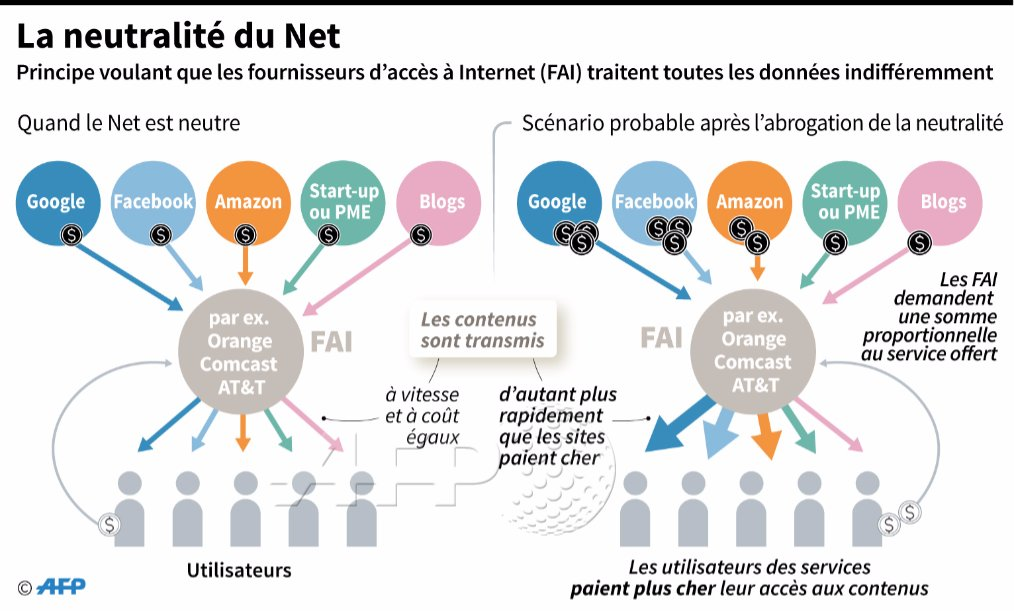
\includegraphics[width=12cm]{neutralite.png}
\end{center}

\subsubsection{Neutralité du Net : quels sont les enjeux ? (Vie Publique, 13 octobre 2020)}\footnote{\url{https://www.vie-publique.fr/eclairage/18846-neutralite-du-net-quels-sont-les-enjeux}}

La neutralité du Net est un principe fondateur d'Internet qui garantit la libre circulation, sans discrimination, des contenus sur le web. % Cette neutralité peut avoir des conséquences importantes non seulement en matière économique (libre concurrence et régulation des acteurs dominants du marché) mais également en termes de respect de la vie privée des internautes, de garantie de la liberté d'expression et de qualité et continuité des services offerts sur Internet.

Internet a été conçu comme un réseau ouvert, reposant sur une architecture décentralisée et le principe du \enquote{meilleur effort} : chaque opérateur doit faire de son mieux pour assurer la transmission de tous les paquets de données qui transitent par son réseau, sans garantie de résultat (obligation de moyen) mais en excluant toute discrimination à l'égard de la source, de la destination ou du contenu de l'information transmise.

%Les principaux acteurs d'internet sont les opérateurs de réseaux (opérateurs de réseaux fixe ou mobile, fournisseurs d'accès à internet) et les fournisseurs de services et de contenus (sociétés telles que Google, Skype, etc.).

%Les utilisateurs d'Internet sont tour à tour récepteurs et émetteurs d'informations ou de services (blogs, réseaux sociaux, Wikipédia, etc.). En bout de réseau, chaque personne a vocation à créer et émettre de l'information (principe du bout à bout). Internet est un réseau universel, partagé par tous et décentralisé. La neutralité d'Internet consiste dans la liberté de transmission au sein de l'architecture communicationnelle d'internet. Cette neutralité de l'Internet est une condition essentielle à son bon fonctionnement et à son développement.

%\section{ La neutralité en France et en Europe }

La loi pour une République numérique du 7 octobre 2016 a inscrit le principe de neutralité de l'Internet dans le droit français. Le principe interdit aux fournisseurs d'accès à internet (FAI) de discriminer l'accès au réseau en fonction des services (par exemple en offrant un internet plus lent à certains clients et plus rapide à d'autres pour accéder à un service identique à partir d'une même offre).

%L'Autorité de régulation des communications électroniques et des postes (Arcep) est garante de la neutralité de l'Internet. Cette neutralité a été consacrée comme principe par le règlement européen du 25 novembre 2015 sur l'Internet ouvert(nouvelle fenêtre), applicable depuis le 30 avril 2016. Pour faire respecter ce principe, la loi du 7 octobre 2016 pour une République numérique a conféré à l'Arcep de nouveaux pouvoirs d'enquête et de sanction à l'encontre des opérateurs.

% Ainsi, l'Arcep a pu faire retirer dans les conditions générales de vente de certains FAI des clauses contraires à la neutralité, qui prévoyaient des blocages de services et de type d'usage (comme l'interdiction du peer-to-peer). L'Arcep rappelle également que des pratiques comme le zero-rating (pratique de certains FAI, en général pour les offres mobiles, consistant à ne pas facturer dans le forfait l'accès à certains sites ou applications) sont contraires au règlement européen. Dans son rapport 2020 sur l'état d'Internet en France(nouvelle fenêtre), l'Arcep considère que le cadre réglementaire qui protège la neutralité du net en Europe a donné les preuves de sa capacité d'adaptation et de sa pertinence pendant la période de confinement.

%Au niveau européen, c'est le Body of European Regulators for Electronic Communications (Berec) qui est chargé de l'application du principe de neutralité du Net.

%Le principe de neutralité du net a été consacré par Cour de justice de l'Union européenne (CJUE) dans une décision du 15 septembre 2020  (CJUE 15 sept. 2020, Telenor, affaires jointes C-807/18 et C-39/19(nouvelle fenêtre)). La Cour a examiné l'application du règlement européen sur l'Internet ouvert par la société hongroise Telenor, fournisseur d'accès à internet, qui proposait un décompte distinct du volume des données consommées selon les applications. Pour certaines applications, les données n'étaient pas comptabilisées (\enquote{tarif nul}) alors que, pour d'autres, des mesures de blocage ou de ralentissement du débit pouvaient être prises en cas de dépassement du forfait. Pour la CJUE, \enquote{de telles offres groupées sont de nature à amplifier l'utilisation des applications et des services privilégiés et, corrélativement, à raréfier l'utilisation des autres applications et des autres services disponibles}. 

%Dans ce cadre, la Cour considère que la société Telenor a enfreint l'obligation générale de traitement égal et non discriminatoire du trafic énoncée à l'article 3 du règlement européen 2015/2120 sur la neutralité du Net. \enquote{Les exigences de protection des droits des utilisateurs d'Internet et de traitement non discriminatoire du trafic s'opposent à ce qu'un fournisseur d'accès à Internet privilégie certaines applications et certains services au moyen d'offres faisant bénéficier ces applications et services d'un \enquote{tarif nul} et soumettant l'utilisation des autres applications et services à des mesures de blocage ou de ralentissement.}

%\section{ Les enjeux économiques et sociaux de la neutralité du Net }

%Un précédent président de l'Arcep, Jean-Ludovic Silicani, considérait que sous l'apparence d'une question très technique ou, à l'inverse, très théorique, ce sujet \enquote{est un des plus fondamentaux que notre économie et notre société aient à traiter au cours des prochaines années, au niveau de chaque pays comme au plan mondial… [car] le bon fonctionnement des réseaux de communications électroniques et de l'internet va constituer une des questions clés de l'avenir de notre planète. Une crise de ces réseaux hypothéquerait l'ensemble des activités et conduirait à un dérèglement général de l'économie et de la société}.

%Les opérateurs d'internet disposent de moyens technologiques qui autorisent une gestion discriminatoire des flux d'informations et peuvent constituer des entraves à la neutralité du net. Ces moyens permettent d'analyser les contenus (de procéder ainsi à la priorisation, au filtrage ou au blocage de certains contenus) et d'organiser leur circulation à plusieurs vitesses.

Les opérateurs de réseau qui militent en faveur de l'abandon de la neutralité justifient ces restrictions d'un point de vue financier. Elles permettraient de dégager des marges de financement supplémentaires requises pour les investissements dans les réseaux.

De même, des gouvernements tentent de mettre en place des techniques de filtrage du réseau pour rétablir un contrôle sur l'information d'Internet, à l'image de celui dont ils jouissent sur les médias traditionnels.

Cependant, la préservation de la neutralité d'Internet est d'abord un enjeu démocratique. La neutralité du net met les citoyens sur un pied d'égalité et permet à tous de s'exprimer librement. Internet est une plateforme d'expression égalitaire qui se distingue à cet égard des moyens de communication traditionnels (radio, TV, presse) car aucun investissement n'est requis pour émettre de l'information.

L'internet ouvert présente, de plus, des enjeux économiques et apparaît comme un incubateur d'innovations. Face aux groupes commerciaux prestataires de services, n'importe quelle petite entreprise peut distribuer librement des services sur Internet et entrer en concurrence sur le marché global. Internet est propice à \enquote{l'innovation sans permis}, des start-up peuvent distribuer à moindre coût et sans autorisation préalable de la part de l'opérateur toute innovation.

%Enfin, Internet contient son propre principe de développement et présente, par là même, d'importants enjeux en matière d'investissement dans l'innovation. En effet, l'enrichissement et l'innovation croissante des services et contenus proposés par internet favorisent l'augmentation du nombre d'utilisateurs.

%Garantir le principe de neutralité d'internet n'équivaut pas à refuser toute pratique de gestion du trafic. Des exigences légales, l'utilisation d'internet devant se faire dans le cadre de la loi, mais également techniques autorisent des atteintes ciblées, temporaires et transparentes au principe de neutralité d'internet sans le remettre en cause (par exemple, blocage des sites avec des contenus pédopornographiques, etc.).

\subsubsection*{Questions}

\begin{enumerate}
  \item Qu'est-ce que la neutralité du net ?
  \item Parmi les exemples suivant, lesquels ne respectent pas la neutralité du net ?
    \begin{enumerate*}[(A)]
      \item Un fournisseur d'accès à internet bloque le traffic en pair-à-pair.
      \item Un fournisseur d'accès à internet diffuse Netflix plus vite que Youtube, suite à un accord commercial avec Netflix.
      \item Un fournisseur d'accès à internet fait payer un accès « prioritaire » au réseau en cas de congestion du réseau.
      \item Un fournisseur d'accès à internet interdit à ses utilisateurs et utilisatrices de télécharger plus de 20Go de données par mois.
      \item Un fournisseur d'accès à internet pratique des prix différents pour ses abonnés en France et en Belgique.
      \item Un fournisseur d'accès à internet propose une offre gratuite ne permettant de visiter que Facebook et Wikipédia.
      \item Un opérateur de téléphonie mobile bloque l'utilisation de Skype en 4G ou 5G.
      \item Un opérateur de téléphonie mobile compresse les images pour accélérer le débit.
      \item Un opérateur de téléphonie mobile fait payer plus cher les appels vers d'autres pays.
      \item À la demande d'un juge, un fournisseur d'accès à internet bloque un site web permettant de téléchargement illégal.
\end{enumerate*}

\item Pourquoi certains fournisseurs d'accès à internet sont-ils opposés à la neutralité du net ?
\item Comment certaines grosses entreprises comme Google ou Facebook pourraient-elles bénéficier de l'abandon de la neutralité du net ?
\item Expliquer pourquoi la neutralité du net permet \enquote{l'innovation sans permis} ?
\item Que signifie : \enquote{aucun investissement n'est requis pour émettre de l'information} ? En quoi la neutralité du net est-elle un enjeu démocratique ?
\end{enumerate}

\end{document}
